\documentclass[preprint]{aastex}
%\documentclass[iop,onecolumn]{emulateapj}

\usepackage{verbatim}
\usepackage{color}
\usepackage[normalem]{ulem} % for striking out with \sout
% A comment block

%\newcommand{\comment}[1]{}

% For color
\newcommand{\mpname}[1]{#1_color.eps}
\newcommand{\clraitoff}{red}
\newcommand{\lumblack}{(black)}
\newcommand{\lumblue}{(blue)}
\newcommand{\lumred}{(red)}
\newcommand{\vdisred}{(red-dashed curve)}
\newcommand{\vdisblue}{(blue-solid curve)}

% For bw
%\newcommand{\mpname}[1]{#1.eps}
%\newcommand{\clraitoff}{}
%\newcommand{\lumblack}{}
%\newcommand{\lumblue}{}
%\newcommand{\lumred}{}
%\newcommand{\vdisred}{(dashed curve)}
%\newcommand{\vdisblue}{(solid curve)}

\newcommand{\umag}{$u$}
\newcommand{\gmag}{$g$}
\newcommand{\rmag}{$r$}
\newcommand{\imag}{$i$}
\newcommand{\zmag}{$z$}
\newcommand{\gmr}{$g-r$}



\newcommand{\gammat}{$\gamma_T$}
\newcommand{\gammacross}{$\gamma_\times$}
\newcommand{\deltasig}{$\Delta \Sigma$}
\newcommand{\deltaplus}{$\Delta \Sigma_+$}
\newcommand{\deltacross}{$\Delta \Sigma_\times$}
\newcommand{\deltarho}{$\Delta \rho$}
\newcommand{\movr}{$M(<r)$}
\newcommand{\sigmacrit}{$\Sigma_{crit}$}

\newcommand{\photoz}{photo-z}
\newcommand{\photozs}{photo-zs}

\newcommand{\tlum}{$L^{tot}$}
\newcommand{\tngal}{$N_{gal}^{tot}$}

\newcommand{\lstarlim}{$0.4 L_*$}
\newcommand{\lvir}{$L_{200}$}
\newcommand{\nvir}{$N_{200}$}
\newcommand{\rvir}{$r_{200}^{gals}$}

\newcommand{\ngal}{$N_{gal}$}
\newcommand{\maxbcg}{maxBCG}
\newcommand{\numNgalBins}{12}
\newcommand{\numLumBins}{16}

\newcommand{\tngalAperture}{2$h^{-1}$ Mpc}

\newcommand{\photo}{\texttt{PHOTO}}
\newcommand{\astrop}{\texttt{ASTRO}}
\newcommand{\mt}{\texttt{MT}}
\newcommand{\spectro}{\texttt{SPECTRO}}
\newcommand{\spectroone}{\texttt{SPECTRO1d}}
\newcommand{\spectrotwo}{\texttt{SPECTRO2d}}
\newcommand{\target}{\texttt{TARGET}}

\newcommand{\lenszmax}{0.3}
\newcommand{\lenszmin}{0.05}

\newcommand{\photoversion}{\texttt{v5\_4}}

%\def\eone{e$_1$}
%\def\etwo{e$_2$}
\newcommand{\etan}{e$_+$}
\newcommand{\erad}{e$_\times$}
\newcommand{\eclass}{\texttt{ECLASS}}
\newcommand{\eclasscut}{-0.06}
\newcommand{\gmrcut}{0.7}

\newcommand{\hrs}{$^{\mathrm h}$}
\newcommand{\minutes}{$^{\mathrm m}$}

\newcommand{\ugriz}{$u, g, r, i, z$}
\newcommand{\polarization}{polarization}

\newcommand{\wgm}{$w_{gm}$}
\newcommand{\wgg}{$w_{gg}^p$}
\newcommand{\wmm}{$w_{mm}$}
\newcommand{\xigg}{$\xi_{gg}$}
\newcommand{\ximm}{$\xi_{mm}$}
\newcommand{\xigm}{$\xi_{gm}$}

\newcommand{\numspec}{127,001}
\newcommand{\numspecvlim}{10,277}
\newcommand{\numrand}{1,270,010}
\newcommand{\numspectot}{278,192}
\newcommand{\numvdis}{49,024}
%\newcommand{\numsource}{10,259,949}
% hirata: 
\newcommand{\nummask}{1,815,043}
\newcommand{\numTenMpc}{132,473}
\newcommand{\numThirtyMpc}{101,221}
\newcommand{\numsource}{27,912,891}

\newcommand{\numpairsTenMpc}{2,670,898,177}
\newcommand{\altnumpairsTenMpc}{2.7 billion}
\newcommand{\numpairsThirtyMpc}{14,818,082,122}
\newcommand{\altnumpairsThirtyMpc}{14.8 billion}



\newcommand{\xirmax}{$\xi_{gm}(R_{max})$}


\newcommand{\localbias}{10-15\%}
\newcommand{\worstlensbias}{XXX\%}
\newcommand{\modelrmin}{15.0}
\newcommand{\modelrmax}{29.0}
\newcommand{\rmin}{15.0}
\newcommand{\rmax}{21.8}
\newcommand{\pofz}{$P(z$)}
\newcommand{\Nofz}{$N(z$)}
\newcommand{\nwei}{N(z)_{\rm wei}}
\newcommand{\npz}{N(z)_{\rm p(z)}}
\newcommand{\nphot}{N(z)_{\rm phot}}
\newcommand{\contamworst}{10\%}
\newcommand{\nphoto}{58,533,603}
\newcommand{\ntrain}{{\color{red} UNKNOWN}}
\newcommand{\matchrad}{2 arcsec}
\newcommand{\cc}[1]{\textcolor{red}{[{\bf Carlos}: #1]}}
\newcommand{\rachel}[1]{\textcolor{green}{#1}}
\def\eps@scaling{1.0}% 

\slugcomment{Last revision \today}
\shortauthors{Sheldon}
\shorttitle{DR8 Photoz Catalog}

\begin{document}

\title{Photometric Redshift Probability Distributions \\for Galaxies in the SDSS DR8}

\author{
Erin S. Sheldon\altaffilmark{1}
}

\altaffiltext{1}{Brookhaven National Laboratory, Bldg 510, Upton, New York 11973}


\begin{abstract}

We present redshift probability distributions for galaxies in the SDSS DR8
imaging data.  We used the weighting algorithm presented in
\citet{LimaPhotoz08} and \citet{CunhaPhotoz09} to derive the overall redshift
distribution \Nofz\ for galaxies with \rmag$ < $\rmax.  The training sample
with redshifts is substantially larger than that used in the DR7 release; of
particular note is addition of the PRIMUS catalog, which is the the most
important training set used in this analysis. With this technique, weights are
calculated for a set of training galaxies with known redshifts such that their
density distribution in five dimensional color-magnitude space is proportional
to that of the photometry-only sample, producing a nearly fair sample in that
space.  The \Nofz\ of the photometric sample is then estimated by constructing
a weighted histogram of the training set redshifts.  We also used this same
method to derive redshift probability distributions \pofz\ for individual
galaxies.
%\textcolor{blue}{  The \pofz\ summed over all galaxies is similar but not
%identical to the redshift distribution of the overall sample. We applied a
%correction to the individual \pofz\ so that the summed \pofz\ equals the
%estimated \Nofz } \textcolor{red}{I think the area I marked in blue is too
%much detail for the abstract}.  
We expect the primary source of error is sample variance: the training sets are
drawn from relatively small volumes of space.  Using simulations we estimated
the uncertainty in \Nofz\ at a given redshift is $\sim$ \localbias.  The
uncertainty on calculations using \Nofz\ or \pofz\ depends on the details; we
discuss the case of weak lensing measurements.  The \pofz\ catalog is available
for download through the SDSS website.  

%The \pofz\ should be used with care, and we describe their
%proper use in detail.

\end{abstract}

\section{Introduction} \label{sec:intro}

Photometric redshifts are estimates of redshift derived using broad-band
photometric observables such as magnitudes and colors.  Typically, the set of
observables for a given galaxy are not sufficient to uniquely specify its
redshift, but only a probability distribution, the \pofz.  These \pofz\ are
often relatively broad. For simplicity of use and interpretation, one commonly
uses a single number, the photometric redshift, as the best estimate of a
galaxy's redshift.  As several recent works have shown
\citep{man08,CunhaPhotoz09,wit09,bor10,abr11}, the use of a single number to
represent the \photoz\ leads to biases.  Working with the full \pofz\ for each
galaxy yields better estimates of the overall redshift distribution, $N(z)$,
and can decrease biases in cosmological analysis.  We note that several public
\photoz\ codes exist that can output a \pofz\ per galaxy, e.g.  {\it Le Phare}
\citep{arn99,ilb06}, {\it ZEBRA} \citep{fel06}, {\it BPZ} \citep{coe06}, {\it
ArborZ} \citep{ger10}, and our own nameless method \citep{CunhaPhotoz09}.


In this paper, we describe a \pofz\ catalog for objects detected in the Data
Release 8 of the Sloan Digital Sky Survey III (SDSS DR8).  We use the method of
\citet{CunhaPhotoz09}, which was also applied to SDSS DR7, with improvements in
the training set and photometry.  The DR7 catalog of \cite{CunhaPhotoz09} has
been successfully used in cosmological analysis, allowing, for example, for the
first measurement of the transverse BAO scale derived purely from angular
information, i.e. without using the 3D power-spectrum \citep{car11}  and for
the measurement of the growth of structure using photometric LRGs
\citep{cro11}. 

This paper is organized as follows.  In \S \ref{sec:method} we discuss the
method and in \S \ref{sec:data},\ref{sec:photo},\ref{sec:select} we describe
the data and sample selection. In \S \ref{sec:train} we discuss the training
set and in \S \ref{sec:results},\ref{sec:errors} we show our results and
estimate errors.  In \S \ref{sec:usage}, we discuss the proper usage of these
results. As an example, we discuss the particular case of weak gravitational
lensing calculations.  In section \S \ref{sec:get} we describe the fomat of the
data to be released, and their permanent archival on the SDSS website.
Finally, in \S \ref{sec:summary} we summarize our results.

\section{Method} \label{sec:method}

The algorithm is detailed in \citet{LimaPhotoz08} and \citet{CunhaPhotoz09}.
The method is to derive weights for a training set of spectroscopically
confirmed galaxies such that the distribution of relevant quantities, such as
magnitudes or colors, matches that of a set of galaxies without known
redshifts, henceforth the photometric sample.  Assuming these quantities
correlate with redshift, and are the only relevant quantities for redshift
determination, the resulting weighted redshift histogram is proportional to the
redshift probability distribution \Nofz\ of the photometric sample. 

The weighting provides a key advantage over other training sample methods such
as neural nets.  Forcing the distributions of observables of the two samples to
be proportional essentially creates a ``fair sample'' from the training set.
This helps avoid the biases that can arise when the training and photometric
samples have different properties.  However, this does require that all areas of
observable space populated by the photometric sample are also populated by the
training set, at least at some low level. 



\subsection{Nearest-neighbor \pofz\ redshift estimators}\label{sec:nnpz}

\subsubsection{Weights}

In this section, we briefly review the weighting method\footnote{The weights
and \pofz\ codes are available at {\url
http://kobayashi.physics.lsa.umich.edu/$\sim$ccunha/nearest/}} of
\cite{LimaPhotoz08}, which is required for computing \pofz.  We define the
weight, $w$, of a galaxy in the spectroscopic training set as the normalized
ratio of the density of galaxies in the photometric sample to the density of
training-set galaxies around the given galaxy.  These densities are calculated
in a local neighborhood in the space of photometric observables, e.g.,
multi-band magnitudes.  In this case, the SDSS {\it ugriz} magnitudes are our
observables; in particular we use four colors and the \rmag--band magnitude.
The hypervolume used to estimate the density is set here to be the Euclidean
distance of the galaxy to its $100^{th}$ nearest-neighbor in the training set.

The weights can be used to estimate the redshift distribution of the
photometric sample:
\begin{equation}  
\nwei = \sum_{\beta=1}^{N_{\rm T}} w_\beta \delta(z-z_\beta)~.
\label{eqn:Nzest}
\end{equation}
\begin{comment}
\begin{equation}  
\nwei = \sum_{\beta=1}^{N_{\rm T,tot}} w_\beta N(z_1<z_\beta<z_2)_{\rm T},
\label{eqn:Nzest}
\end{equation}
\end{comment}

\noindent For a bin $z_1 < z < z_2$, we sum the weights of all training
set galaxies that fall within that bin.  
Ref.~\cite{LimaPhotoz08,CunhaPhotoz09} show that this indeed provides
a nearly unbiased estimate of the redshift distribution of the photometric
sample, $N(z)_{\rm P}$, provided the differences in the selection of the
training and photometric samples are solely in the observable quantities used
to calculate the weights.  For example, if the photometric sample
has some sort of shape dependent cut, the same cut should be applied to the
training sample or shape should be one of the observables used to measure
weights.


\subsubsection{\pofz}

To estimate the redshift error distribution for each galaxy, \pofz,
we adopt the method of \cite{CunhaPhotoz09}. The \pofz\ for a given object in the
photometric sample is simply the redshift distribution of the $N$
nearest neighbors in the {\bf training} set.

\begin{equation}
\hat{P}(z) = \sum_{\beta=1}^{N_{\rm nei}} w_\beta \delta(z-z_\beta)~.
\label{eqn:pzest}
\end{equation}

\noindent This is the same as Eqn. \ref{eqn:Nzest} but limited to the nearest
neighbors of a given object.  We choose $N=100$ for this study, and estimate
\pofz\ in 35 redshift bins between $z=0$ and 1.1.  We can also construct a new
estimator for $N(z)_{\rm P}$ by summing the $\hat{P}(z)$ distributions for all
galaxies in the photometric sample,
\begin{equation}
\npz = \sum_{i=1}^{N_{\rm P,tot}}\hat{p}_i(z)~.
\label{eqn:Nhat2}
\end{equation}
\noindent This estimator becomes identical to that of Eqn. (\ref{eqn:Nzest})
in the limit of very large training sets.  For training sets smaller than tens
of thousands of galaxies, one can improve the \pofz s by multiplying each \pofz\ by the
ratio of $\nwei$ to $\npz$.
That is,
\begin{equation} \label{eq:pzcorrect}
P(z) \rightarrow P(z)\frac{\nwei}{\npz} \label{eqn:pzcorrect}
\end{equation}
This correction essentially corresponds to using the weights estimate as a
prior on the \pofz s.



\section{Photometric Data} \label{sec:data}

The photometric data were drawn from data release 8 (DR8) of the Sloan Digital
Sky Survey III.  Full details are given in the data release paper \citet{dr8}.
As compared to the earlier DR7 release, DR8 includes an additional 2500 deg$^2$
of new imaging in the Southern Galactic Cap (SGC), acquired to facilitate
spectroscopic target selection for the \bossfull\ (\boss), which is part of
SDSS III.


SDSS imaging are gathered using the 2.5 meter at Apache Point \citep{Gunn06}
with the camera \citep{Gunn98} running in time-delay-and-integrate mode.
Observations are taken in each of the SDSS bandpasses {\it ugriz} nearly
simultaneously as sky moves across bands in the order $riuzg$.  The data were taken
during photometric nights under relatively good seeing conditions
\citep{Hogg01}.  A series of pipelines are run to calibrate the data
\citep{Nikhil08,Smith02,Tucker06}, derive astrometry \citep{Pier03}, and
calculate fluxes, shapes and other interesting quantities
\citep{LuptonADASS01}.  
Note the calibrations used for these data are derived using the ``ubercalibration''
technique presented in \citet{Nikhil08}.  
\section{Photometric Quantities} \label{sec:photo}

In this section we describe the photometric quantities used in creation of the
input catalog.  Most of these quantities are measured by the SDSS photometric
pipeline \photo. An early version of the pipeline is described in
\citet{LuptonADASS01}.  Other details can be found in the SDSS Data Release
papers, e.g. \citet{dr4} and at the SDSS III website\footnote{\sdssweb}.  We
will give a few additional details below.  Note, in comparison to DR7, the DR8
makes use of an updated version of the \photo\ software reduction pipeline,
v5\_6 rather than v5\_4, including some updates to sky subtraction that can
change galaxy photometry and, potentially, the $P(z)$.

For colors we use the SDSS ``model magnitudes'', which we will refer to as
\modelmag \footnote{\DRatemags}.  Each object is fit to an elliptical
exponential disk and an elliptical \devauc\ profile convolved with a double
Gaussian approximation to the PSF model interpolated to the location of the
object \citep{LuptonADASS01,Sheldon04}.  For the \modelmag, the best fit model
in the \rmag\ band is then used to extract the flux in the other four
bandpasses, accounting appropriately for the PSF in each band. Thus the
effective aperture is the same for all bands, which is appropriate for
extraction of color information.

We use ``composite model magnitudes'' as an approximate total magnitude for
each object, which we will refer to as \cmodelmag.  For each bandpass
separately, the flux from the best-fitting exponential and \devauc\ models are
combined:
\begin{equation}
\textrm{Flux}_{cmodel} \equiv (1-f_{dev})\times \textrm{Flux}_{exp} + f_{dev} \times \textrm{Flux}_{dev}
\end{equation}
where $f_{dev}$ is the fraction of the total flux estimated to come from a
\devauc\ profile.  Note the effective aperture for each band is
different, so these magnitudes are not appropriate for estimating colors.

For quality assurance, we use bits from the \texttt{OBJECT} bitmask output by
\photo \footnote{\DRateflags}.    We also use the \texttt{RESOLVE\_STATUS} to
choose primary observations\footnote{\DRateresolve}.  We will describe how the
flags are used in section \S \ref{sec:select}.


\begin{comment}
\begin{itemize}
  \item \texttt{SATUR}  The object contains saturated pixels.
  \item \texttt{BRIGHT} The object is very bright and must be remeasured.
  \item \texttt{DEBLEND\_TOO\_MANY\_PEAKS}
\end{itemize}
\end{comment}
    

\section{Photometric Sample Selection} \label{sec:select}

\subsection{Star Galaxy Separation} \label{sec:sg}

The \photo\ pipeline uses the concentration $c$ to separate stars from
galaxies.  The concentration is the difference between magnitude determined
from the best fitting PSF model \psfmag\ and the \modelmag\, which is
the better fitting of the exponential and \devauc\ models convolved
with the local PSF:
\begin{equation}
c \equiv \textrm{psfmag} - \textrm{modelmag}~.
\end{equation}
For stellar objects, the scale of the \modelmag\ approaches a delta function and
the result becomes equivalent to the \psfmag.  Thus the concentration should be
$\ge 0$ within the noise, with stars close to zero and galaxies greater than
zero.  The pipeline defines galaxies as objects with $c > 0.145$ where $c$ is
derived from the summed fluxes from all bandpasses\footnote{\DRateclass}.  

At our magnitude limit $r = $\rmax, the stellar contamination may be relatively
large.  Using a small space-based data set matched to SDSS data as a truth
table, the approximate stellar contamination can be determined.  At \rmag\ = 21
the contamination is a few percent, but the contamination increases to
approximately \contamworst\ at \rmag\ = 22\footnote{\DRsevsg}.  

For studies where completeness and purity must be known precisely,
\citet{ScrantonMag05} recommend using probabilistic star galaxy separation at
fainter mags (\rmag\ $ > $ 21); i.e.  attempt to determine the {\it
probability} that an object is a galaxy and either use that as a weight or make
appropriate cuts. 


In practice the end user should perform more strict cuts on the data to choose
a subset that suits their needs.  We provide a catalog here that should be a
superset of objects that can be further trimmed.

\subsection{Other Cuts}

We remove objects for which the extinction-corrected model flux is not well
determined in at least one of the bands.  The magnitude limits are [21, 22, 22,
20.5, 20.1] for \allmag\ respectively.

In addition to the magnitude limits described above, which ensures a reasonable
detection in at least one band, we additionally demand that we have some
detection in both the \rmag\ and \imag\ bands.  Rather than applying a
magnitude cut, we instead use the \texttt{OBJECT} processing flags
\texttt{BINNED}\{1,2,4\}, which indicate the object was detected in the
original image (binned by 1), the $\times$2 binned image, or the $\times$4
binned image respectively.

We remove all objects that are found to have the following \texttt{OBJECT}
flags set: \texttt{SATUR}, \texttt{BRIGHT}, \texttt{DEBLEND\_TOO\_MANY\_PEAKS},
\texttt{PEAKCENTER}, \texttt{NOTCHECKED}, \texttt{NOPROFILE} as well as objects
that are (\texttt{BLENDED} \&\& \texttt{NODEBLEND}); in other words, detected
to be blended but not successfully deblended into components. 

We only use objects marked as \texttt{SURVEY\_PRIMARY} in their
\texttt{RESOLVE\_STATUS} flags field. Different scans on the sky image the same
objects due to the small overlap regions between adjacent scans, overlaps at
the end of the scan lines where the great circles converge, and re-observed
scan lines.  This results in duplicate observations for many objects.  These
duplicates are ``resolved'' and only a single observation is kept.  Note this
primary also implies that, if the object is blended, it is either a child or
not deblended further.  This cut is made in the \texttt{OBJECT} flags as
\texttt{!BRIGHT \&\& (!BLENDED || NODEBLEND || nchild == 0)}.

We require the extinction corrected \citep{Schlegel98} \cmodelmag\ in the \rmag\
band to be in the range [\rmin, \rmax].  We also restrict the extinction corrected
\modelmag\ to be within the range [\modelrmin, \modelrmax] in order to ensure
reasonable colors for the galaxies.

We make broad geometrical cuts on the catalog.  We trim the objects to the
\boss\ footprint, shown in Fig. \ref{fig:footprint}. We also remove any
objects near stars in the tycho2 catalog \citep{tycho2} using a variable radius
that depends on the magnitude of the star:
\begin{equation}
r = (0.0802\times B_T^2 - 1.860\times B_T + 11.625)/60.0
\end{equation}
where $B_T$ is the Tycho magnitude and $r$ is in degrees.  Finally, we remove
all objects from images taken where a \umag\ amplifier was not working\footnote{\DRsevcaveat}.

\begin{figure}[t] \centering
 \centering 
 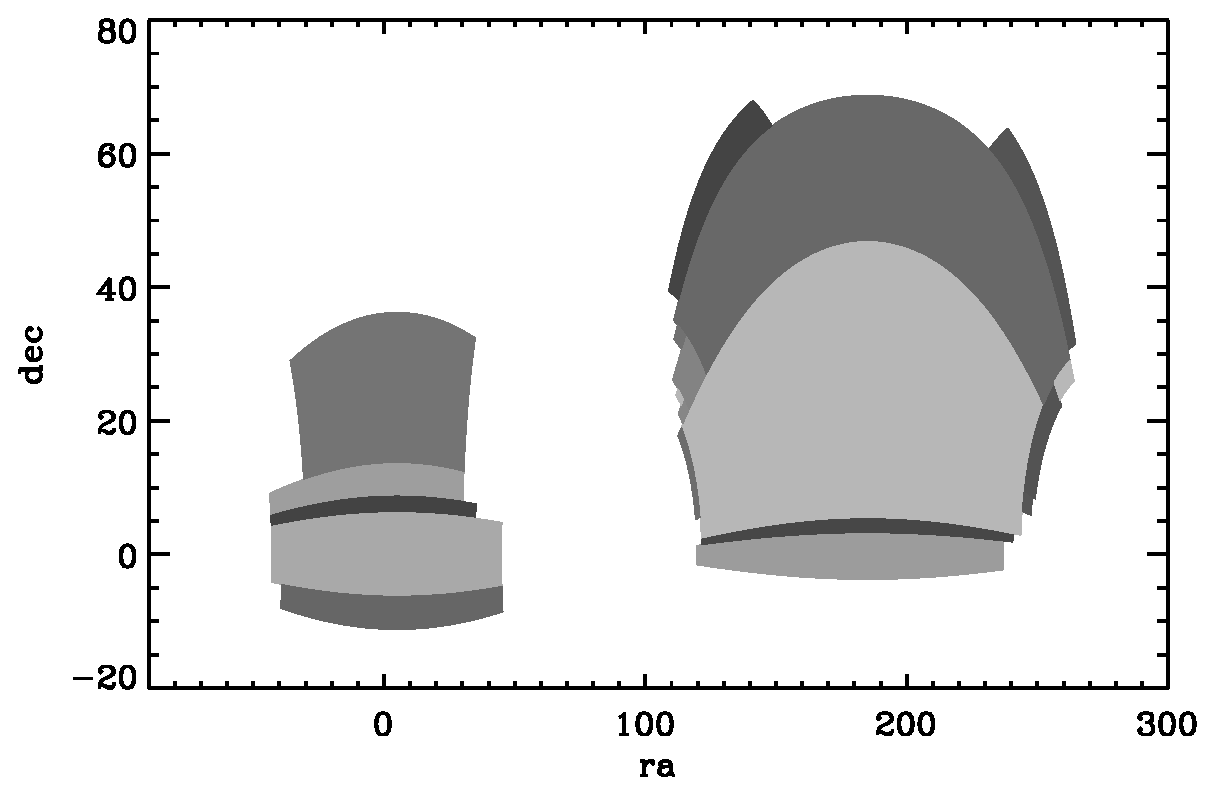
\includegraphics[scale=0.75]{figures/boss-poly-coverage.eps}
 %\plotone{figures/boss-poly-coverage.eps}
 \caption{BOSS footprint for the north galactic cap on the left
 and the south galactic cap on the right.  The differently shaded
 regions represent contiguous rectangular regions in SDSS survey coordinates.
 Note points with RA $>$ 300 have been wrapped below zero 
 to avoid the 360 crossing point.}
 \label{fig:footprint}
\end{figure}

The final photometric catalog contains \nphoto\ objects.  The distributions of
extinction-corrected \rmag-band \cmodelmag\ and colors derived from
extinction-corrected \modelmag\ are shown in Fig. \ref{fig:varhist}.

\section{Training Samples} \label{sec:train}

We use a spectroscopic training set drawn from a number of sources. These
sources contain mostly galaxies and a small number of stars in order to help
characterize stellar contaminants from the photometric sample at low redshift.
In the following sections we give short details on each sample and describe our
process for matching to the photometric sample.

\subsection{Samples Used in this Study} \label{sec:train:def}

\begin{itemize} 

    \item 435,878 redshifts from the SDSS spectroscopic samples,
principally from the \texttt{MAIN} and Luminous Red Galaxy \texttt{(LRG)}
samples, with confidence level \texttt{zconf}$ > 0.9$, and r-band
\cmodelmag\ $ <19.5$.


    \item 445 objects from the Canadian Network for Observational
Cosmology (CNOC) Field Galaxy Survey \cite[CNOC2;][]{yee00}\footnote{\tt
http://www.astro.toronto.edu/$\sim$cnoc/cnoc2.html} with \texttt{Rval} $>4$
for \texttt{Sc}$=2$ or \texttt{Rval} $> 5$ for \texttt{Sc}$=5$

    \item 151 from the Canada-France Redshift
Survey \cite[CFRS;][]{lilly95}\footnote{\tt
http://www.oamp.fr/people/tresse/cfrs/cfrs.html} with \texttt{Class} $\geq 3$.

    \item 1,868 from the Deep Extragalactic Evolutionary Probe 2 survey
\citep[DEEP2;][]{weiner05}\footnote{\tt http://deep.berkeley.edu/DR3}
with \texttt{zqual} $\geq 3$. 
Of these, 1,499 are an approximately magnitude-limited sample from the Extended Groth Strip (EGS).
The remainder is $BRI$ color-selected to target $z>0.7$ galaxies, hereafter called the non-EGS sample. 

    \item 197 from the Team Keck Redshift Survey \cite[TKRS;][]{wirth04}\footnote{\tt http://tkserver.keck.hawaii.edu/tksurvey/}.

    \item 8,633 LRGs from the 2dF-SDSS LRG and QSO Survey \cite[2SLAQ;][]{cannon06}\footnote{\tt http://www.2slaq.info/} with \texttt{qop} $\geq$ 3.

    \item  2,080 from zCOSMOS redshift survey \cite{lilly07}, with  \texttt{cc=3.4 || 3.5 || 4.4.  || 4.5 || 9.5}.
    
    \item 1,587 from the VIMOS VLT-Deep survey \cite[VVDS;][]{garilli08}\footnote{\tt http://www.oamp.fr/virmos/vvds.htm} with \texttt{zqual} $\geq 3$.

    \item 16,874 from four fields of the PRIMUS survey
    \cite[PRIMUS;][]{coil10,cool12}\footnote{\tt
    http://cass.ucsd.edu/$\sim$acoil/primus/}.  Only PRIMUS objects with $Q$ ==
    4 were used.      \end{itemize}

\subsection{Matching to SDSS Imaging Data} \label{sec:train:match}

We spatially match the training sets listed in \S \ref{sec:train:def} to the
photometric catalog described in \S \ref{sec:select}.  We choose the closest
match within \matchrad.  By performing this match we place the training set
galaxies on the same photometric system as the photometric set.  We also
guarantee that the matches are drawn from the same magnitude range, and have
the same quality cuts applied, as the photometric set.

As noted in \S \ref{sec:train:def}, the training sets contain some stars.
There are also some stars in the photometric set, since the star galaxy
separation is not perfect.  Thus, through this matching between photometric set
and training set it should be possible to place some fraction of the stars in
the photometric set at redshift zero; or at least some part of their derived
\pofz.

\section{Results} \label{sec:results}

We use the algorithm described in \S \ref{sec:method} to derive weights for
each training set galaxy.  We then use these weights to calculate a weighted
redshift histogram which, under our assumptions, should be proportional to that
of the photometric set.  We also derive individual redshift probability
distributions \pofz\ for each photometric galaxy.

\subsection{Derived Weights in Observable Space}

The \rmag-band \cmodelmag\ and colors based on \modelmag\ for the photometric
and training sets are shown in Fig. \ref{fig:varhist}.  Also shown are the
derived weights for the training set and the resulting weighted histograms.
These are the fundamentally new calculations we present in this work.

The weighted training set distributions should be approximately proportional to
the photometric set distributions in order to derive good redshift
distributions.  There are deviations at \gmr\ $\sim 1.5$ and \rmi\ $\sim 0.6$,
but qualitatively the distributions are close.  It may be possible to learn
something by comparing these distributions directly, but we will instead focus
on the accuracy of the recovered redshift distributions.

\begin{figure}[p] \centering
    %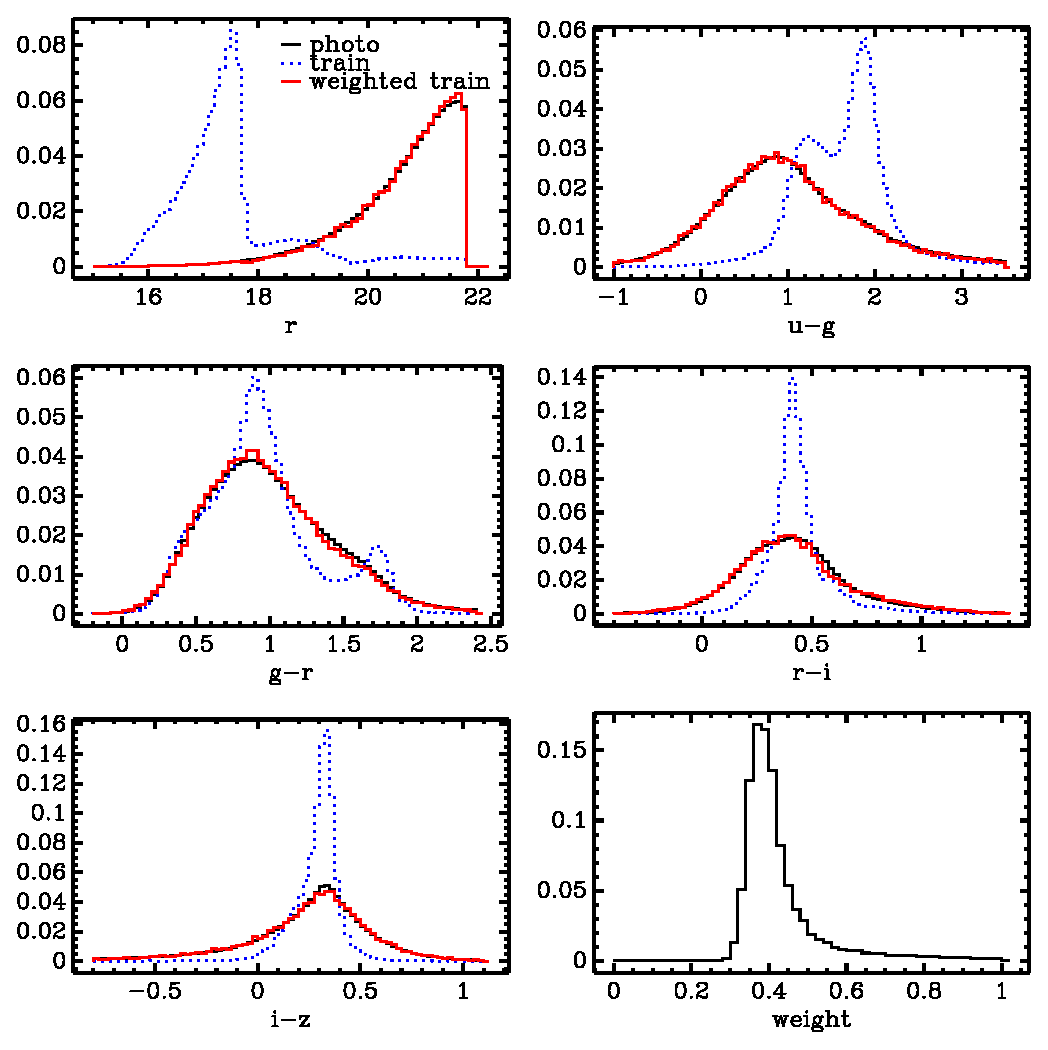
\includegraphics[scale=0.5]{figures/zweight-10-varhist.eps}
    \plotone{figures/zweight-10-varhist.eps}

    \caption{Distributions of photometric quantities for the photometric sample
    and training sample.  The upper left panel shows the extinction-corrected
    \rmag-band \cmodelmag.  Note both samples are cut at \rmag$ < $\rmax.  
    Also shown is the weighted histogram for the training sample where
    the weights are derived to produced distributions approximately 
    proportional to the photometric sample.
    The following four panels show extinction-corrected colors based on
    \modelmag.  The bottom right panel shows the distribution of of the
    derived weights for the training sample. }
    \label{fig:varhist}

    \vspace{2em}
\end{figure}

\subsection{Derived \Nofz}

Figure \ref{fig:pofz} shows the recovered redshift distribution for the entire
\rmag\ $<$ \rmax\ sample.  Also shown is the redshift distribution of the
original training set.  These distributions are in qualitative agreement with
those shown in \citet{CunhaPhotoz09}, although that sample had a fainter
\rmag-mag limit at 22.0.  Note the sub-plot showing the region near $z=0$.  As
expected there is some fraction of the overall distribution near z=0.  The
fraction of the probability at $z < 0.002$ is about 0.4\%.  It is not known exactly how many
stars are in the photometric sample, but this is probably a lower limit on the
stellar contamination (see \S \ref{sec:sg}).  We will estimate the errors on
this distribution in \S \ref{sec:errors}. These \Nofz\ data are presented in
Table \ref{tab:nofz}.


\subsection{Derived \pofz}

Also shown in Fig. \ref{fig:pofz} is the summed \pofz\ derived for individual
galaxies.  The uncorrected $\npz$\ is, characteristically, slightly more peaked than
than $\nwei$.
In \S \ref{sec:pzcorr} we apply Eq. \ref{eqn:pzcorrect} to correct the \pofz s.

\begin{figure}[p] \centering
    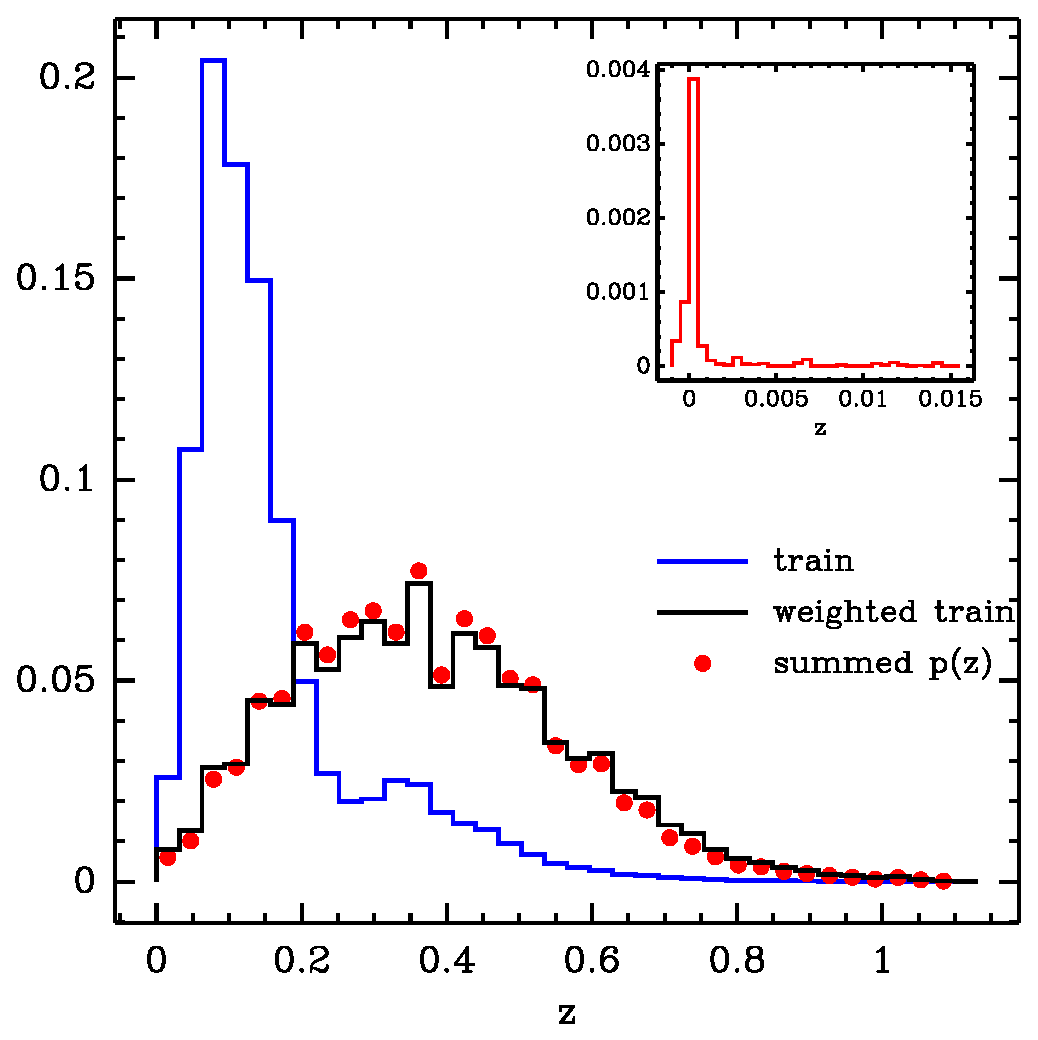
\includegraphics[scale=0.9]{figures/zweight-10-zhist-withorig-withsum-12.eps}
    %\plotone{figures/zweight-10-zhist-withorig-withsum-12.eps}

    \caption{Reconstructed redshift distribution for SDSS galaxies with \rmag\
    $ < $ \rmax.  The overall reconstructed distribution, shown in red, is
    derived by creating a weighted histogram of the training set redshifts as
    described in the text.  Also shown in magenta is the sum of all \pofz\
    derived for individual galaxies.  The unweighted training set redshift
    distribution is shown in blue.  The expected errors on these distributions
    from cosmic variance in the training set is shown in Fig.
    \ref{fig:ebars}. The excess at $z \sim 0$ is due to stars in training set
    having significant weight; more detail at low redshift is shown in the
    inset.  This excess is at least partly due to the presence of real stars in
    our photometric sample resulting from imperfect star-galaxy separation.
    The fraction of the distribution at $z < 0.002$ is 0.4\%, which is probably
    a lower bound on the stellar contamination.  \label{fig:pofz}}

    \vspace{2em}
\end{figure}

In Fig. \ref{fig:rand6pofz} we show 6 randomly chosen \pofz.  Each panel
contains a random \pofz\ drawn from a particular magnitude range in extinction-corrected
$r$-band \cmodelmag; these ranges are given in the figure caption.
This figure captures the general trend that the \pofz\ are broader at
fainter magnitudes.

\begin{figure} [t]\centering
    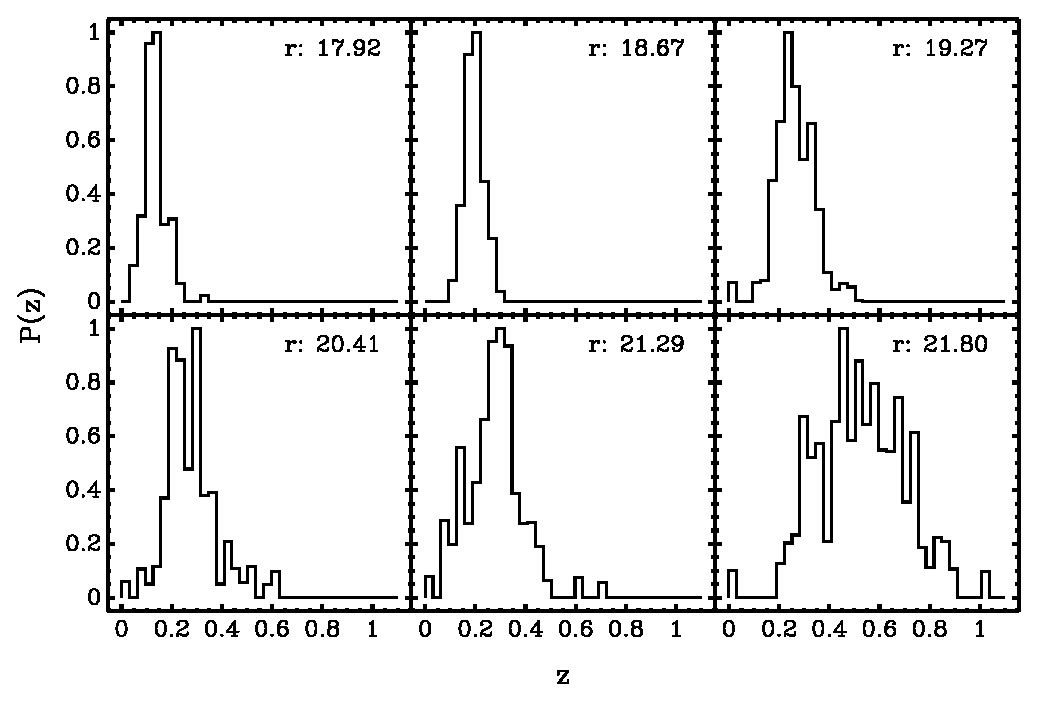
\includegraphics[scale=0.7]{figures/seed25-5-6pofz.eps}
    %\plotone{figures/11-6pofz.eps}
    \caption{Randomly chosen \pofz.  For each panel, a random object was
    chosen from a particular magnitude range.  Column-wise from top the
    left these ranges are $[r < 18], [18 < r < 19], [19 < r < 20], 
    [20 < r < 21], [21 < r < 21.5], [21.5, < r < 21.8]$.  
    The extinction-corrected $r$-band \cmodelmag\ of each object
    is indicated in the upper right of each panel.
    \label{fig:rand6pofz}}
\end{figure}

The uncertainty in individual \pofz s is typically dominated by shot-noise
error.  The scale of both statistical and systematic uncertainties in the
individual \pofz s is strongly correlated with the width of the \pofz\
\citep{CunhaPhotoz09}.  A broader \pofz\ reflects a larger degeneracy in
observable space, and requires more training-set objects to characterize.  Fig.
\ref{fig:pzwidth} shows the distribution of objects in the photometric sample
as a function of \rmag-band magnitude and $1-\sigma$ width of the \pofz.  The
contours indicate factor of 2 changes in density.  

We recommend using the $1-\sigma$ or other width measures of the \pofz\ as the
most efficient way to trim the sample for improved precision and accuracy.  The
\pofz\ width should also be a reasonable error estimator for use with other
\photoz\ methods.  However, we discourage using the peak or some other single
number statistic derived from the \pofz\ as a proxy for redshift. See 
\S \ref{sec:usage} for more details.
\begin{comment} If a single-number \photoz\ estimate is needed we recommend
using a neural network or nearest-neighbor polynomial based approach
\cite[e.g.][]{Oyaizu08}.  \end{comment}

\begin{figure}[p]\centering
    %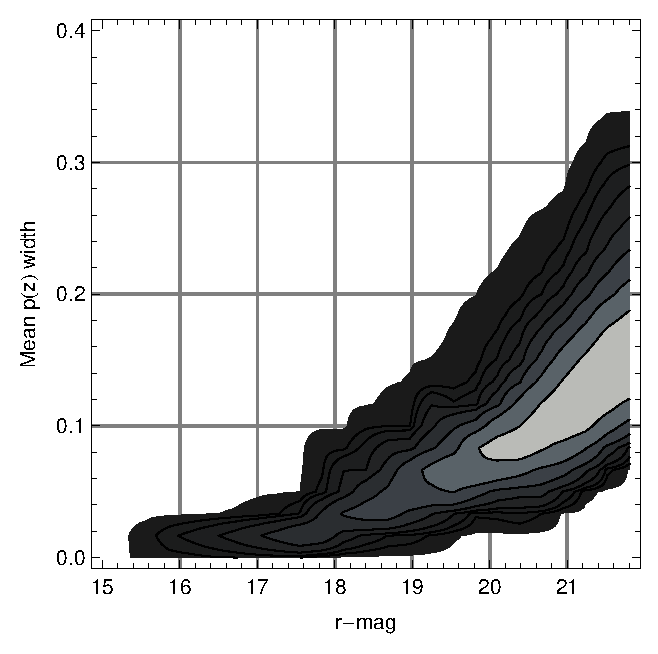
\includegraphics[scale=0.8]{figures/pzwidth25bins.eps}
    \plotone{figures/pzwidth25bins.eps}
    \caption{Density contours of the mean \pofz\ width as a function of {\it r} magnitude. 
The width of each \pofz\ is the defined as the standard deviation about the mean. 
The contours represent factors of 2 changes in density.}
    \label{fig:pzwidth}
    \vspace{2em}
\end{figure}

\subsubsection{Correction to \pofz} \label{sec:pzcorr}

As we will demonstrate in \S \ref{sec:pofp}, the individual \pofz\ appear to be
somewhat less accurate than the overall \Nofz.  We can correct the individual
\pofz\ to agree, in the mean, with the overall \Nofz\ using Eqn.
\ref{eqn:pzcorrect}.  This correction factor is shown in Figure
\ref{fig:pzcorr}.  Note at $z \gtrsim 0.9$ neither the \Nofz\ or the summed
\pofz\ are well constrained, and the correction factor is noisy.  For $z > 0.9$
we use the average correction from that range.

\begin{figure}[t]\centering
    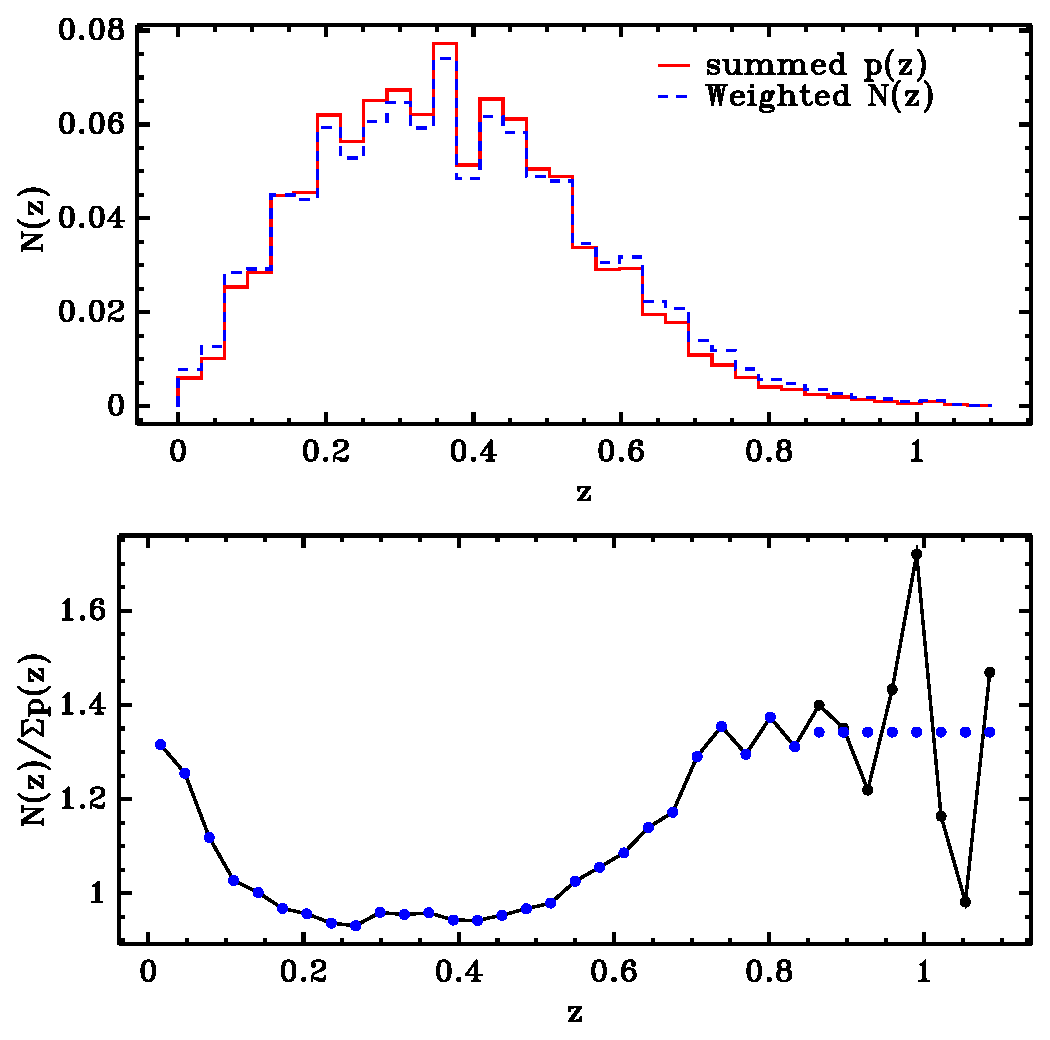
\includegraphics[scale=0.6]{figures/pofz-correct-12.eps}
    %\plotone{figures/pofz-correct-12.eps}

    \caption{Correction factor from Eq. \ref{eqn:pzcorrect}.  This correction
    factor is the ratio of the \Nofz, which we find to be unbiased, to the summed
    \pofz\ from individual objects. The top panel shows both \Nofz\ and \pofz\
    and the bottom panel is the ratio.  We apply this correction to each of the
    \pofz\ in the release catalog.  Note for $z > 0.9$ we use the average
    correction from that range.}

    \label{fig:pzcorr}
    \vspace{2em}
\end{figure}



\section{Sources of Error} \label{sec:errors}

As detailed in \cite{CunhaPhotoz09}, the derived weights, and inferred \Nofz,
are susceptible to at least four kinds of training-set selection effects:
spectroscopic failures, large-scale structure bias (sample variance + shot
noise in the training set), and selection in non-photometric observables.  In
addition, the fact that the weights use a non-infinitesimal volume in color-magnitude
space to re-weight the photometric set can yield a small Eddington bias to the
recovered distribution.  And, as mentioned previously, incorrect star-galaxy
separation can result in incompleteness and contamination of the sample.
Because our training set consists of many different surveys with different
characteristics, it is important to quantify the contribution of each to the
overall result.  Table \ref{tbl:weistats} lists, for each of the surveys
comprising the training set, the number of objects, the approximate area, and
the percentage the survey contributes to the weighted estimate of the overall
redshift distribution.  This percentage is calculated by summing up the weights
assigned to objects in each survey and dividing by the sum of weights from the
entire training set.


From Table \ref{tbl:weistats}, we see that PRIMUS carries the most weight by a
large margin at 62\%.  Overall, the magnitude limited surveys that reach our
selection depth of \rmax\ - PRIMUS, TKRS, CNOC2, DEEP2-EGS, CFRS, VVDS, and
zCOSMOS - represent about 81$\%$ of the total weight.  
This is desirable,
because it minimizes the risk of bias in our assessment of errors in what follows.
The Table also shows that the SDSS MAIN sample ($r<17.8$) contributes only $1.7\%$ of the weights, which
is consistent with the fraction expected from simulations for a flux-limited sample 
to $r<21.8$.
The remainder of the SDSS spectra are LRGs to $r<19.4$, which make a more
substatial contribution to the total weight at 7.4\%.

In what follows, we identify potential sources of systematics and detail our
tests to constrain them:

\begin{itemize}

\item {\it Large-scale structure: } We expect this to be the main source of
error.  We use galaxy+$N$-body simulations\footnote{Simulations provided courtesy of Risa Wechsler and
Michael Busha. See \cite{bushasimulations} for details.}
 to estimate the sample variance plus shot
noise uncertainties of the spectroscopic redshift distributions of the training
set.  For simplicity, we only simulate the magnitude limited surveys of the
training set.  In addition, because of the overlap between zCOSMOS and one of
the PRIMUS fields, we neglect the zCOSMOS sample in the error estimation to
simplify the calculation.  This results in a $\sim$10\% increase in the error
bars relative to including zCOSMOS as an independent sample.  The predicted
error bars are overlayed on the simulated overall redshift
distribution in Fig.
\ref{fig:ebars}.  The errors are also given in Table \ref{tab:nofz}. The
uncertainty in the training set redshift distributions is not identical to that
of the uncertainties in the estimated redshift distributions \Nofz\ derived using
the weights, hence the error bars should be used only for a reasonable
reference.  A more detailed estimation of the errors would require SDSS-specific
photometry+$N$-body simulations.  Relative to the error bars in the
training set, the error bars in the weighted N(z) should be (very roughly)
about 20-30\% smaller, with increased anti-correlations between neighboring
bins, but to be certain would require more detailed investigation.
%There are also 
We explore these issues in more detail for a different data set
in \citet{CunhaPhotozLSS11}.


\item {\it Selection in non-observables: } Two of the surveys comprising our
training set have selections in observables that are not included in the SDSS
magnitude limited sample.  As mentioned previously, the DEEP2-nonEGS sample is
selected using BRI photometry to target galaxies above $z>0.7$.  As shown in
\citet{CunhaPhotoz09}, the use of DEEP2 in earlier versions of this catalog
resulted in a bump in the overall estimated redshift distribution around $z\sim
0.8$.  The present data release has a brighter magnitude cut and additional
training data, which has eliminated this bias.  
Now, DEEP2-nonEGS carries about 1.4\% of the total weight.  The 2SLAQ sample targets
LRG's.  Besides SDSS magnitudes, it also uses morphological information in the
selection.  Because shape correlates poorly with redshift, biases due to inclusion of the
2SLAQ sample are expected to be small.  2SLAQ is an important part of our
sample because it provides a better training set for LRG's at higher redshift
than the SDSS sample.

\item {\it Spectroscopic redshift failures: } The impact of spectroscopic failures is the
most difficult to quantify.  We chose a bright $r$-magnitude cut, and relatively
stringent cuts on spectroscopic quality to minimize effects of failures, but it
is possible that errors due to spectroscopic failures are not negligible.
% but it
%is possible that some features seen in the redshift distribution - such as the
%dip around $z=0.4$ are due partly to spectroscopic failures.
%{\color{red} this seems speculative, can we say anything quantitative?  If not
%perhaps simplify the comment to ``it is possible that there are significant
%errors due to spectroscopic failures''.}

\item {\it Seeing: } \citet{Nakajima11} point out that differences
between the seeing distribution of the galaxies in the photometric and the
training set can lead to biases in the \photoz\ error calibration.  In figure
\ref{fig:seeing} we show the seeing distributions for all of our photometric
sample compared to the four highest weight training samples, not including SDSS
for which the seeing distribution is a near perfect match.  The distributions
are qualitatively similar, but with a trend to better seeing for the training
set matches.  More quantitatively, we checked the sensitivity of our results to
seeing-induced biases by including seeing as a variable in the weights
estimation.  We find only negligible change in the recovered redshift
distribution.  Hence, although differences in seeing are in general a concern, we
find little effect in our data.
\end{itemize}

For individual $P(z)$, the main source of uncertainty is shot-noise, because
only 100 galaxies were used to estimate each $P(z)$.  The choice to fix the
number of neighbors keeps the shot-noise equal for all galaxies, but can also
yield biases or an artificial broadening of the $P(z)$ if the training set is
too sparse near the galaxy of interest.  However, we do not find the volume
spanned by the 100 nearest neighbors to be a good indicator of the $P(z)$
quality. This is because other properties of the redshift-observable
hypersurface affect the local density of galaxies.  A potentially more
interesting indicator of bias in individual $P(z)$ is the spatial distribution
of the training set nearest neighbors relative to the galaxy for which a $P(z)$
is needed.  We leave these explorations for a future work.

%The bias due to sparse training set manifests itself as a difference between 
%the summed $P(z)$ and the weights estimate of the $N(z)$. 
%We fin


\begin{figure}[h]\centering
    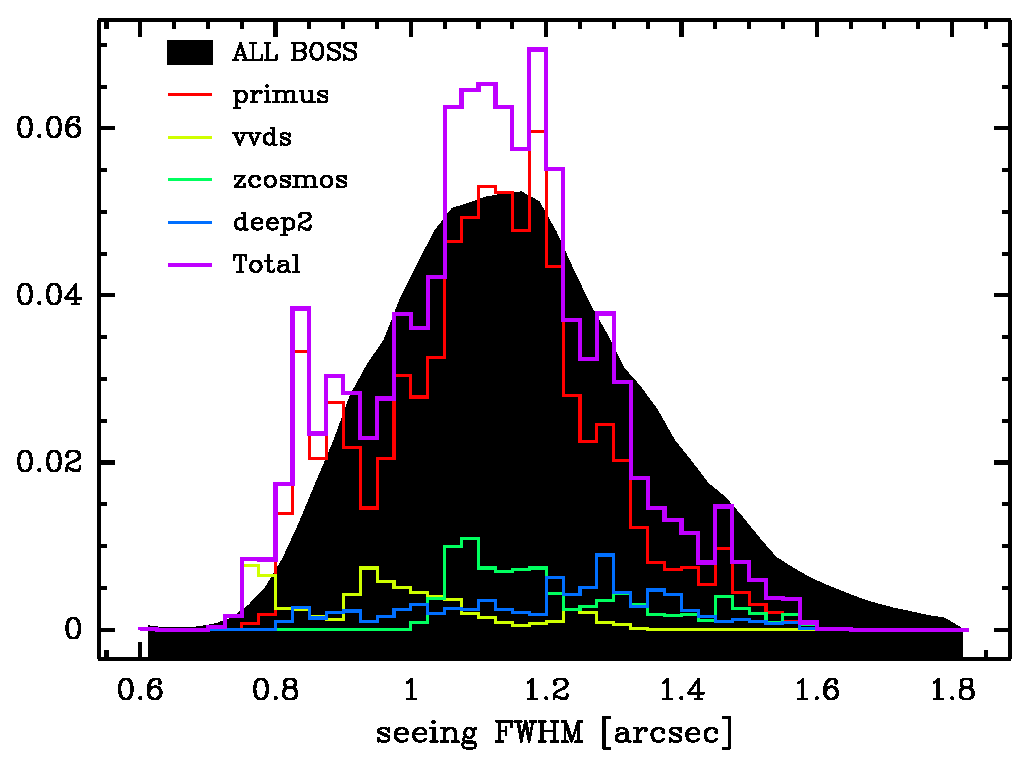
\includegraphics[scale=0.7]{figures/primus-vvds-zcosmos-deep2-match-seeing-10.eps}

    \caption{Distribution of seeing for the photometric sample (All BOSS) and
    the four most important training samples.  These samples are important
    because they are magnitude limited and give relatively high weight in the
    analysis.  Also shown is the sum of the training samples.  The curves for
    each sample are normalized relative to the summed curve.  The summed and
    photometric curves are normalized to unity.}

    \label{fig:seeing}
\end{figure}

\begin{figure}[t]\centering
    %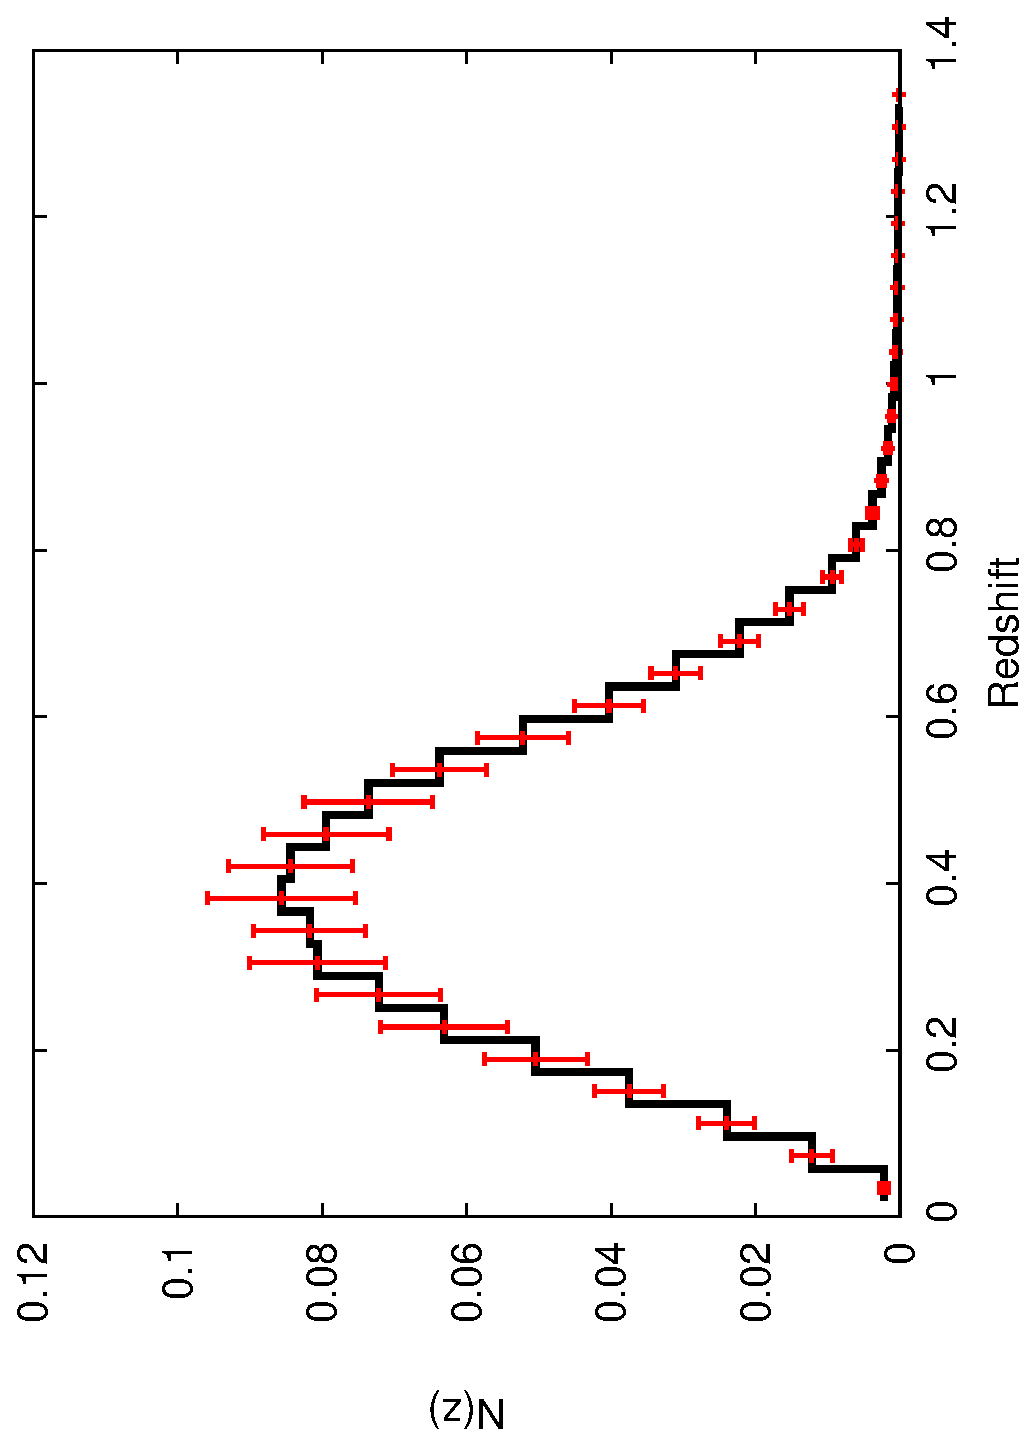
\includegraphics[{angle = -90,scale=0.5}]{figures/nz.sim.error.eps}
    %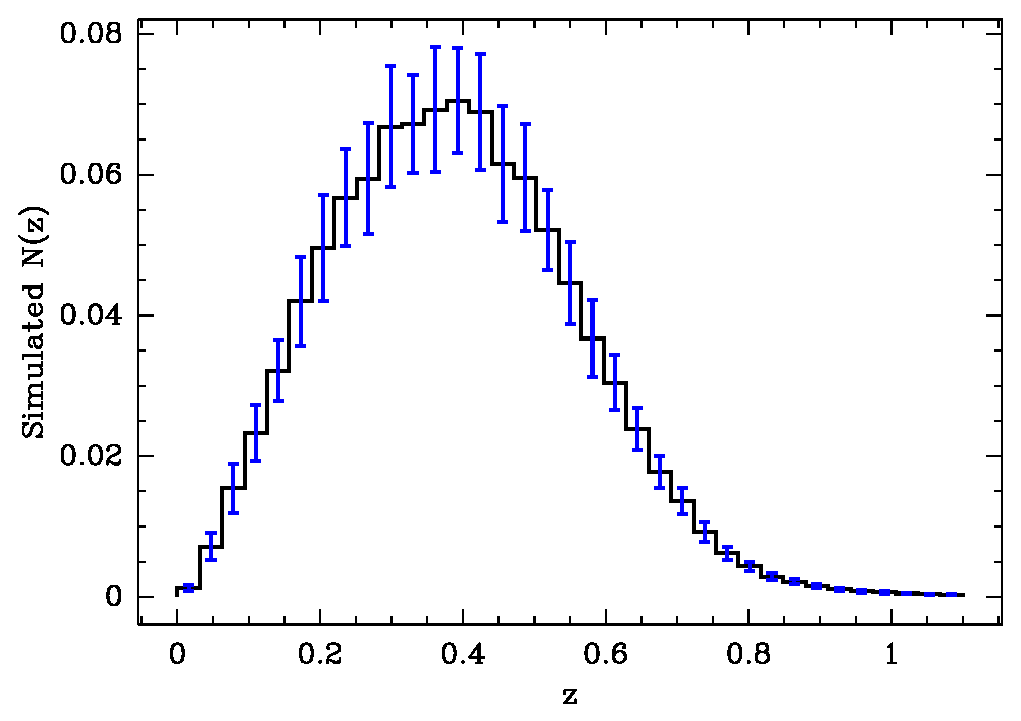
\includegraphics[scale=0.7]{figures/nzsigf-edges-errblue.eps}
    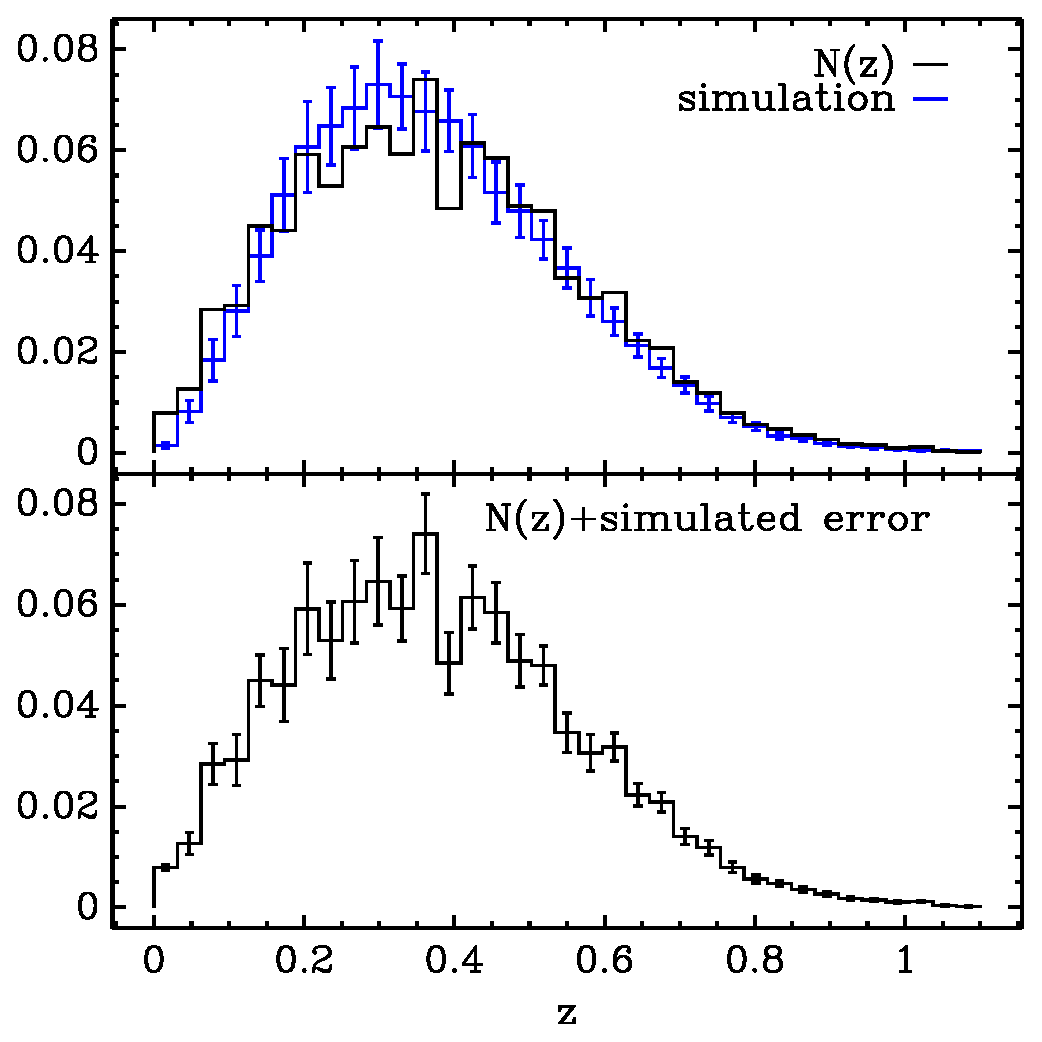
\includegraphics[scale=0.6]{figures/nzsigf-edges-12-nofz-sim-errors-2panel.eps}

    \caption{Top panel: Simulated redshift distribution with errors for an
    $r$-band $<$ \rmax\ sample.  The error bars are the $1-\sigma$ simulated
    variability due to sample variance in the catalogs comprising the training
    set.  Also shown is the estimated \Nofz\ for our sample.  Lower panel:
    estimated \Nofz\ combined with the predicted sample variance errors from
    the simulation.}

    \label{fig:ebars}
    \vspace{2em}
\end{figure}

%}

\begin{deluxetable}{lrrr}
\tablecaption{Statistics for Each Training Set \label{tbl:weistats}}
\tablewidth{0pt}
\tablehead{
    \colhead{Survey} &
    \colhead{Number of Objects} &
    \colhead{Area} &
    \colhead{Weight Fraction}
}
\
\startdata
PRIMUS$^*$          &16,874   &5.2     & 63\% \\
2SLAQ               &8,633    & 180    & 6.0\%\\
TKRS$^*$            &197      & 0.07   & 0.55\%\\
CNOC2$^*$           &445      &0.4     & 1.6\%\\
DEEP2-EGS$^{*}$    &1,499    & 0.4    & 5.8\%\\
DEEP2-nonEGS$^{*}$ &369      & 2.8    & 1.4\%\\
SDSS                &435,875 &DR5      & 7.4\%\\
SDSS ($r < 17.8$)       &376,625 &DR5      & 1.7\%\\
CFRS$^*$            &151     & $<$0.1  & 0.76\%\\
VVDS$^*$            &1,587   &4.0      & 6.0\%\\
zCOSMOS$^*$         &2,080   &1.7      & 7.5\% 
\enddata
\tablecomments{Number of galaxies, area in square degrees, and fractional contribution to the 
weights estimate of $N(z)$. The ``*'' indicates samples that are approximately flux-limited to our
selection depth. }
\end{deluxetable}

\begin{comment}
\begin{table}[!ht]
\caption{{\color{red}We should use deluxetable and add a caption}}
\label{tbl:weistats}
\begin{center}
\begin{tabular}{ l r r r }\hline \hline
Survey & Number of objects & Area$deg^2$ & Weight fraction \\ \hline 
PRIMUS$^*$ &14,196 &5.2 & 62\% \\
2SLAQ  &8,577 & 180 & 7.0\%\\
TKRS$^*$  &151  & 0.07& 0.50\%\\
CNOC2$^*$ &412  &0.4 & 1.8\%\\
DEEP2-EGS$^{*!}$ &1,075  & 0.4 & 3.5\%\\
DEEP2-nonEGS$^{*!}$ &301  & 2.8 & 2.7\%\\
SDSS &435,878  & & 9.1\%\\
CFRS$^*$ &122  & $<$0.1 & 0.67\%\\
VVDS$^*$ &1,771  &4.0  & 5.5\%\\
zCOSMOS$^*$ &1,247 &1.7  & 7.4\% \\ \hline \hline
 %\multicolumn{2}{c |}{Survey} & \multicolumn{2}{| c}{Parameter Uncertainty} \\ \hline
%Original Parameters & New Parameters & $\sigma(\DE)$ & $\sigma(w)$ \\ \hline
%free & free & 0.8662 & 0.4206 \\
%\multicolumn{2}{l}{add Planck priors} & 0.0331 & 0.1078 \\
%\multicolumn{2}{l}{Planck priors} & 0.0331 & 0.1078 \\
%free & sharp & 0.0142 & 0.0456 \\
%sharp & sharp & 0.0024 & 0.0110 \\ \hline
\end{tabular}
\end{center} 
\end{table}
\end{comment}



\section{Proper Use} \label{sec:usage}

In this section we describe the proper use of these redshift distributions.
We risk an overly pedantic discussion here in order to ensure that past
mistakes are not repeated by the uninitiated.

If one desires to use the \pofz\ to evaluate any non-linear function $F(z)$,
one must integrate the function times the \pofz\ over the entire distribution;
i.e. one must take the expectation value of the function.  The reason is quite
simple. In general a function evaluated at the expectation value of $z$ does not
equal the expectation value of the function:
\begin{equation}
\langle F(z) \rangle \ne F(\langle z \rangle).
\end{equation}
The expectation value of the function should be computed as follows:
\begin{equation}
\langle F \rangle = \int_{0}^{\infty} F(z) P(z) \mathrm{d}z.
\end{equation}
It is {\bf not} correct to simply take the effective redshift $\int
z\,P(z)\,\mathrm{d}z$ and evaluate
the function at that redshift.

This is true in most interesting science cases.  An excellent example is in
gravitational lensing, where one must estimate the ``critical surface density''
\sigmacrit, which determines the lensing strength of a given lens-source pair; the
lensing deflection angle is proportional to \scinv.  The function
\sigmacrit\ depends on the angular diameter distances to the lens, source and
between lens and source in a non-linear way.  The proper estimator for a lens
at redshift $z_{l}$ and source with $P(z_s)$ is
\begin{equation} \label{eq:calcscrit}
\Sigma^{-1}_{\mathrm{crit}}(z_l) = 
    \int_{0}^{\infty} \Sigma_{\mathrm{crit}}^{-1}(z_l, z_s) P(z_s) \mathrm{d}z_s.
\end{equation}


\subsection{\pofz\ and galaxy-galaxy lensing: proof-of-principle} \label{sec:pofp}

Particular analysis techniques may be more or less sensitive to the width of
\pofz\ or other properties of \pofz\ or \Nofz.  In this section, we use the
galaxy-galaxy lensing calibration method from \cite{man08} and
\citet{Nakajima11} as an example of determining this sensitivity.
This methodology requires the use of a fair subsample of source galaxies with
spectroscopic redshifts.  For the purpose of this paper, we use the DEEP2 EGS
region, in which there are 730 galaxies that (a) pass all cuts to be included
in the SDSS source catalog from \citet{MandelbaumSystematics05}, (b) have
secure redshifts from DEEP2, and (c) pass the additional cut $r<21.5$.

Note, DEEP2 EGS is only one of the many training samples used in our analysis.
So this should be thought of as a proof-of-principle.

In brief, the quantities that we have measured are the expected calibration
bias $b_z$ in the galaxy-galaxy lensing signal due to the method of estimating
the source redshift (i.e., a multiplicative systematic error), and the degree to
which the variance in the lensing signal deviates from the ideal variance we
would achieve with optimal weighting by the true source redshift (large
deviation results in increased statistical error).  The increase in statistical
error when we have degraded redshift information comes both from source
misidentification, and also from deviations of the weights from the
optimal\footnote{Optimal weighting would also include a factor that downweights
galaxies with noisier shape measurements, $\propto (e_\mathrm{rms}^2 +
\sigma_e^2)^{-1}$.  For simplicity, we neglect this factor in the tests that
follow; however, in order to use this weighting, which modifies the effective
$N(z)$, the shape measurement error weighting must also be used in the
derivation of the $P(z)$ from the training sample.} $1/\Sigma_\mathrm{crit}^2$.
Schematically, these two quantities can be determined via weighted sums over
lens-source pairs $j$ (with weight $\tilde{w}_j$; in what follows, estimated
quantities using approximate redshift information have a tilde, and ones that
use the true redshift do not):

\noindent
\begin{equation} \label{eq:lensbias}
b_z + 1 = \frac{\sum_j \tilde{w}_j (\tilde{\Sigma}_{\mathrm{crit},j}
   / \Sigma_{\mathrm{crit},j})}{\sum_j \tilde{w}_j}
\end{equation}
and
\begin{equation} \label{eq:lensweight}
\textrm{Variance ratio}  \equiv \frac{\textrm{Ideal variance}}{\textrm{Real
     variance}} = \frac{(\sum_j \sqrt{\tilde{w}_j w_j})^2}{(\sum_j
     w_j)(\sum_j \tilde{w}_j)}.
\end{equation}
For more detail, see the aforementioned papers.

In Figure \ref{fig:simplebias} we show the results of these calculations for
several test cases.  First, the red short-dashed curve gives, as a baseline,
the calibration bias (top) and variance ratio (bottom) when using the ZEBRA
\photoz\ studied in \citet{Nakajima11}.  As shown, there is a
significant bias in the lensing signal that must be calibrated out.
Next, the green long-dashed line shows what happens if we use the
$N(z)_\mathrm{wei}$ as an estimate of the redshift distribution, rather than
using any individual galaxy \photoz\ or $P(z)$ information.  Crucially, the
lensing signal is unbiased in this case. However, as shown in the bottom
panel, we do find an increased
statistical error due to lack of redshift information on a per-galaxy basis.

Third, the solid black line shows what happens when we use the individual
$P(z)$ to estimate $\Sigma_\mathrm{crit}$ using Eq. \ref{eq:calcscrit}.  These
$P(z)$ are derived from a very specific, idealized case, using {\em only} EGS
both as the training sample and the photometric sample.  In this case, the
individual $P(z)$ are on average $40\%$ broader than the DR8 $P(z)$ because of
the use of 100 neighbors to construct the $P(z)$ when the training sample
itself is only $7$ times as large.  To compensate for the bias introduced by
the small size of the training sample, we have imposed a multiplicative
correction factor to the $P(z)$ such that $\sum P(z) = N(z)_\mathrm{wei}$ using
Eq. \ref{eq:pzcorrect}.  Nonetheless, there is a calibration bias due to the
very significant width of the $P(z)$ (which can be removed using a calibration
sample); but the variance ratio is still far closer to optimal than when we did
not use weighting information, and slightly closer than when we used ZEBRA
\photoz.  

The magenta dot-dashed line shows the results when 7 neighbors are used to
estimate the \pofz, not including the galaxy itself. The blue dot-long dashed
line shows the same case but with the Eq.~\ref{eq:pzcorrect} correction.  This
use of 7 neighbors reduces the abnormally broad $P(z)$ caused by using such a
small training sample and 100 neighbors.  The mean $P(z)$ width for the 7
neighbors case is 0.0989, to be compared to the mean width of the DR8 $P(z)$ of
0.0983. The calibration bias for 7 neighbors is also quite close to the ideal
case with $N(z)_\mathrm{wei}$, and the weighting is the closest to optimal of
all the cases considered in this paper.

To summarize, we have demonstrated for this simplified training set that, for
the purpose of lensing, we achieve a perfect signal calibration when using
$N(z)_\mathrm{wei}$; i.e. no individual galaxy redshift information.  However,
the weighting is suboptimal.  When we use individual $P(z)$, the lensing signal
can be biased due to their finite width even if $\sum P(z) =
N(z)_\mathrm{wei}$, but this bias can be calibrated out.  The advantage of
using individual \pofz\ information is that statistical errors on the lensing
signal are reduced due to more optimal weighting.  This is because a
signal-to-noise ratio weighting goes as $\langle \Sigma_{\mathrm{crit}}^{-2}
\rangle$, so sources expected to be behind the lens are given higher weight
than those expected to be close to or in front of the lens.

Again, we emphasize that this analysis used only DEEP2 EGS, and should be used
as a proof-of-principle to gain intuition.  Users of these data should perform
similar analyses to these but matched to their exact analysis and selection
criteria.

\begin{figure} [h]\centering
    \includegraphics[scale=0.5]{figures/pz.egs.c3n7.paper.ps}

    \caption{ Proof of concept analysis of errors in a fictitious lensing
    analysis.  For this example we used only DEEP2-EGS galaxies but perfect
    weights estimate; the sample variance, and width of individual \pofz, are
    much larger than for the DR8 analysis.  {\em Top:} Lensing signal
    calibration bias (Eq.  \ref{eq:lensbias}) as a function of lens redshift,
    for four  cases labeled on the plot and discussed in the text.  {\em
    Bottom:}  Ratio of the ideal to the real signal variance when using
    different  methods of redshift determination; the goal is to stay as close
    to $1$  as possible. \label{fig:simplebias}}

\end{figure}



\section{Acquiring the Data} \label{sec:get}

{\color{red} Give the data model and location  of files on DR8 website. }

\section{Summary} \label{sec:summary}

In this paper we presented a catalog of photometric redshift probability distributions for
the SDSS DR8.  This catalog uses the same method as the \pofz\ catalog for SDSS
DR7 presented in \cite{CunhaPhotoz09}, with some modifications.  For this
catalog, we use the ubercal photometry.  We also add the PRIMUS galaxy sample,
which more than doubles the number of galaxies in our training set that are
drawn from a flux-limited sample other than SDSS.  The addition of PRIMUS
provides a significant increase in the total area of the non-SDSS training set, which
helps to reduce sample variance.  We examined several potential sources of
error, including shot noise, sample variance, seeing, star-galaxy separation,
and spectroscopic failures.  We expect that sample variance is the main source
of uncertainty in our overall redshift distribution.  For individual \pofz s,
shot-noise is the limiting uncertainty, since each \pofz\ is based on 100 training set galaxies.  
Differently from the DR7 catalog, we
did not use repeat observations of our training set galaxies.  The use of
repeats can provide more localized and smoother \pofz\ estimates, and are often
useful.  However, because only part of our sample had repeat observations, the
use of repeats would effectively increase the sample variance of our results.
The use of repeats may be beneficial for LRGs because the training set is not
sample variance limited in this case.  We may release a catalog trained on
repeat observations at a future date.  

\begin{deluxetable}{cccc}
\tablecaption{Estimated \Nofz\ and Sample Variance Errors \label{tab:nofz}}
\tablewidth{0pt}
\tablehead{
    \colhead{zmin} &
    \colhead{zmax} &
    \colhead{\Nofz} &
    \colhead{Sample Variance Error}
}
\
\startdata
0.000000 & 0.031428 & 0.007881 & 0.000449 \\
0.031429 & 0.062857 & 0.012669 & 0.001953 \\
0.062857 & 0.094285 & 0.028415 & 0.003462 \\
0.094286 & 0.125714 & 0.029208 & 0.003958 \\
0.125715 & 0.157143 & 0.044956 & 0.004287 \\
0.157143 & 0.188571 & 0.044070 & 0.006356 \\
0.188572 & 0.220000 & 0.059196 & 0.007557 \\
0.220000 & 0.251428 & 0.052931 & 0.006892 \\
0.251429 & 0.282857 & 0.060654 & 0.007913 \\
0.282857 & 0.314285 & 0.064638 & 0.008631 \\
0.314286 & 0.345714 & 0.059264 & 0.006961 \\
0.345715 & 0.377143 & 0.074072 & 0.008895 \\
0.377143 & 0.408571 & 0.048450 & 0.007447 \\
0.408572 & 0.440000 & 0.061471 & 0.008265 \\
0.440000 & 0.471428 & 0.058448 & 0.008265 \\
0.471429 & 0.502857 & 0.048904 & 0.007633 \\
0.502857 & 0.534285 & 0.047974 & 0.005717 \\
0.534286 & 0.565714 & 0.034663 & 0.005862 \\
0.565715 & 0.597143 & 0.030663 & 0.005484 \\
0.597143 & 0.628571 & 0.031781 & 0.003876 \\
0.628572 & 0.660000 & 0.022291 & 0.002934 \\
0.660000 & 0.691428 & 0.020855 & 0.002284 \\
0.691429 & 0.722857 & 0.014056 & 0.001832 \\
0.722857 & 0.754285 & 0.011847 & 0.001407 \\
0.754286 & 0.785714 & 0.007948 & 0.000930 \\
0.785715 & 0.817143 & 0.005635 & 0.000698 \\
0.817143 & 0.848571 & 0.004771 & 0.000544 \\
0.848572 & 0.880000 & 0.003537 & 0.000392 \\
0.880000 & 0.911428 & 0.002684 & 0.000288 \\
0.911429 & 0.942857 & 0.001806 & 0.000236 \\
0.942857 & 0.974285 & 0.001517 & 0.000204 \\
0.974286 & 1.005710 & 0.001030 & 0.000156 \\
1.005710 & 1.037140 & 0.001150 & 0.000126 \\
1.037140 & 1.068570 & 0.000423 & 0.000106 \\
1.068570 & 1.100000 & 0.000146 & 0.000104
\enddata

\tablecomments{Reconstructed redshift distribution \Nofz\ for SDSS galaxies
with \rmag\ $ < $ \rmax.  The first two columns specify the redshift range of
the bin and the third is the reconstructed \Nofz. The fourth is the sample
variance errors derived from simulations, which we expect to be the dominant
uncertainty.  These sample variance errors should be thought of as a somewhat
rough estimate.  A more perfect match would require a simulation more
specifically tuned to the SDSS data.}

\end{deluxetable}


%Summarize what we did.  Compare to other estimators?

%- Compare to DR7 p(z)'s: Added PRIMUS, no repeats-> focus on decreasing sample variance, UBERCAL, Payed attention to the seeing.

%- Previous usage in the literature. Mandelbaum et al, Carnero et al, Crocce et al (, Liu et al, 

%- Abrahamse: mathematical proof that P(z)'s are unbiased if N(z) is correct.





\bibliographystyle{apj}
% Bib database
\bibliography{apj-jour,astroref}



\end{document}

